\section{Presentazione del modello di business}

Per la vendita del nostro prodotto crediamo che la cosa migliore sia rivolgersi direttamente al cliente finale. Per questo prevediamo la realizzazione di un e-commerce per la vendita diretta al cliente e, nel primo periodo, la vendita anche su store già noti come Amazon per avere un bacino di utenti più ampio e farsi conoscere ai primi clienti. Oltre alla vendita online, che crediamo sia quella per noi più importante, prevediamo di intraprendere delle partnership con aziende produttrici di vasi per la vendita di bundle vaso+PotNet.

I costi di produzione stimati per singola unità, considerando solo i materiali, saranno compresi tra i 5 gli 8 euro, con un prezzo di vendita ipotizzato tra i 25 e i 30 euro.

Dopo un primo periodo iniziale, prevediamo di realizzare una nuova versione di PotNet con un numero di sensori maggiore e funzionalità. Questo, a fronte di un costo di produzione di poco maggiore (1-2€), ci permetterà di vendere questa nuova versione ad un prezzo tra i 35 e i 40 euro, quindi con un utile superiore rispetto alla prima versione.

Oltre a questo, saranno presenti dei piani di abbonamento a cui gli utenti potranno sottoscriversi per ottenere funzionalità aggiuntive sul bot Telegram e sulla Web UI. Prevediamo di lanciare questi abbonamenti ad un prezzo abbastanza basso, intorno ai 2-3 euro, in modo da convincere più clienti possibile a sottoscriversi.

Il nostro modello di business si basa quindi sui ricavi provenienti dalla vendita del prodotto, i quali però generano un'entrata per l'azienda solo una volta, e dalla sottoscrizione dei clienti ad abbonamenti aggiuntivi, i quali prevedendo rinnovi mensili, genereranno per l'azienda un flusso di entrate più costante nel tempo.

\begin{figure}[ht!]
	\centering
	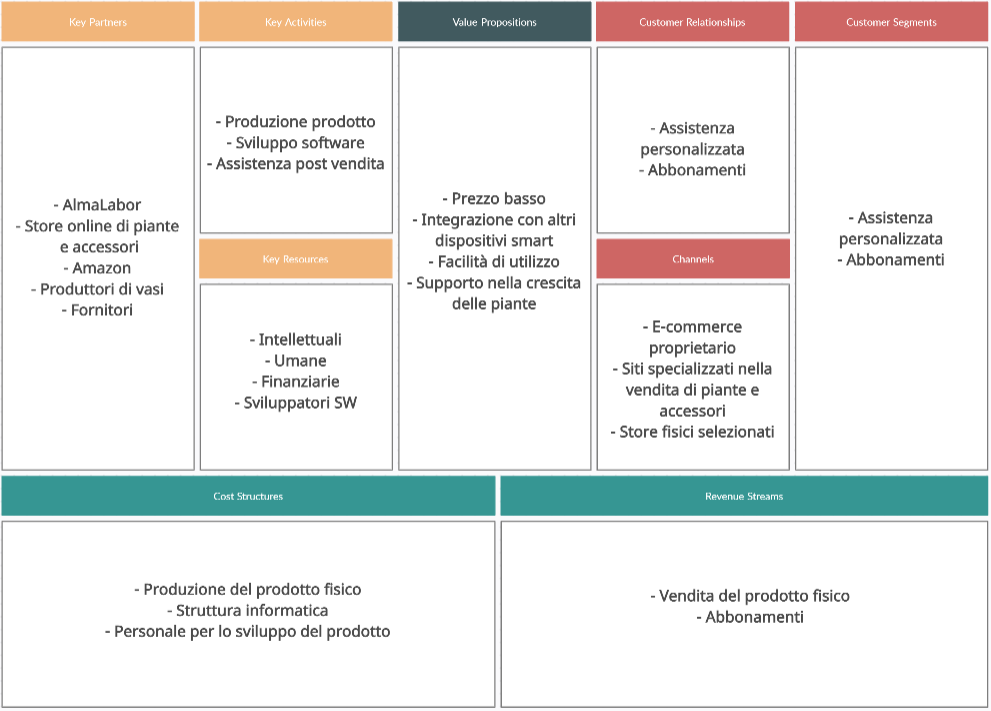
\includegraphics[width=\textwidth]{./images/Business-Model-Canvas.PNG} 
	\caption{Business Model Canvas \label{overflow}}
\end{figure}